\icode{N-MD-CA-L2-260627-001}
如图，质量为\(M=\) \,\qty{2.5}{kg}的一只长方体形空铁箱在水平拉力\(F\)作用下沿水平面向右匀加速运动，铁箱与水平面间的动摩擦因数\(\mu_1\)为0.3。这时铁箱内一个质量为\(m=\) \,\qty{0.5}{kg}的木块恰好能静止在后壁上、木块与铁箱内壁间的动摩擦因数\(\mu_2\)为0.25。设最大静摩擦力等于滑动摩擦力，\(g\)取\,\qty{10}{m/s^2}。求：
\begin{enumerate}
    \item 木块对铁箱的作用力大小；
    \item 铁箱和木块一起运动的加速度；
    \item 水平拉力\(F\)的大小；
\end{enumerate}
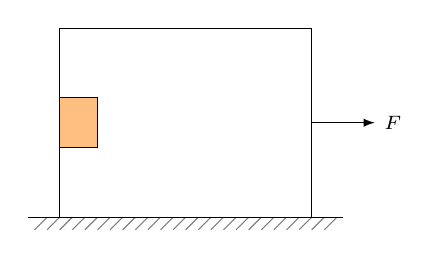
\begin{tikzpicture}[scale=.8,>=latex,font=\scriptsize]
    \draw (0,0) rectangle(4,3);
    \draw[fill=orange!50] (0,1.1) rectangle(.6,1.9);
    \draw[->] (4,1.5)--(5,1.5)node[right]{\(F\)};
    \foreach \x in{-.4,-.2,...,4.3}
      \draw[gray] (\x,-.2)--++(.2,.2);
    \draw (-.5,0)--(4.5,0);  
\end{tikzpicture}